\newpage\section{Application}
	\subsection{Presentation}
	
	Here we will present the look of our application, and describe its functionnalities. In the \textsc{Figure} \ref{fig:general} we can see the welcoming screen of the guide.
	It has :
	\begin{enumerate}
		\item A title;
		\item A data entering zone;
		\item A welcoming map.
	\end{enumerate}
		\begin{figure}[h!]
			\centering
			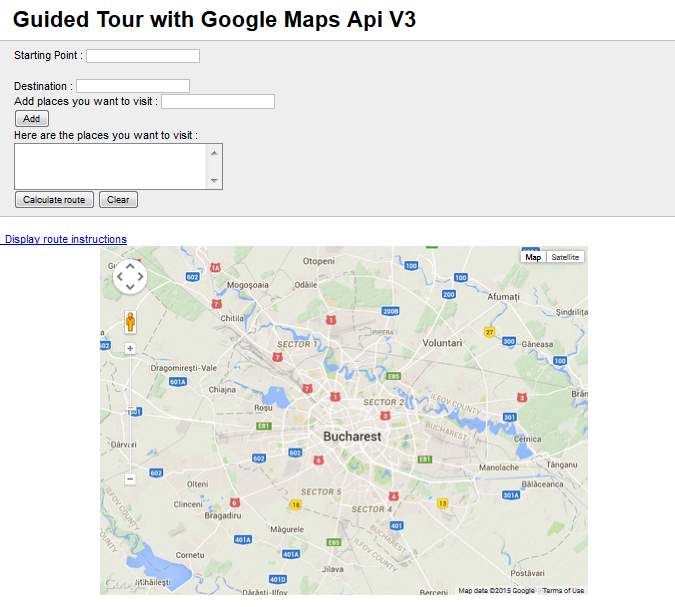
\includegraphics[scale=0.7]{input/general_look.png}
			\caption{\label{fig:general}General look of the application.}
		\end{figure}
		The map provided by the Google Maps API is directly loaded when the page is open. It focuses by default on Bucharest.
		
		\newpage If HTML5 geolocation is not enabled by default on your browser, or if you ask for each time a website wants to access if, you may see the pop-up in \textsc{Figure} \ref{fig:geoloc}, asking you to enable this feature.
		\begin{figure}[h!]
			\centering
			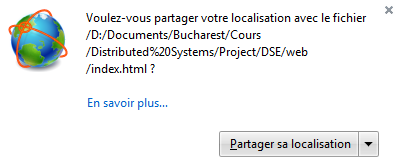
\includegraphics{input/geoloc.png}
			\caption{\label{fig:geoloc}Pop-up asking for your location.}
		\end{figure}
		
		If you decide to enable it, the welcoming map will display your position, as shown in the \textsc{Figure} \ref{fig:geoloc_map}.
		\begin{figure}[h!]
			\centering
			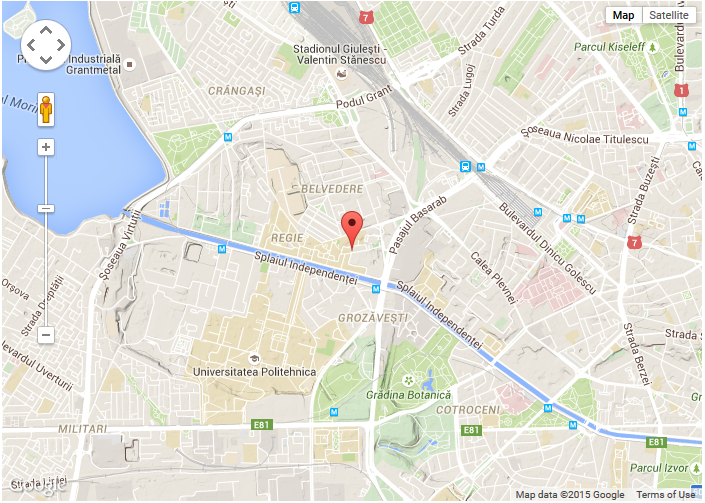
\includegraphics[scale=0.7]{input/geoloc_map.png}
			\caption{\label{fig:geoloc_map}Map showing your position.}
		\end{figure}
		
		Once the welcoming page reached, you can start using the application. It is very simple, you should follow these steps :
		\begin{enumerate}
			\item Enter a starting point;
			\item Adding an arrival point;
			\item Add the intermediate points you want to reach by entering them one by one, and clicking the \textit{Add} button.
			\item Click the \textit{Calculate button}
		\end{enumerate}
		Note that the order in which you enter the intermediate points does not matter, the way will be optimized during the calculation phase.
		There is a \textit{Clear} button to clear this list in case you made a mistake.
		
		\begin{figure}[h!]
			\centering
			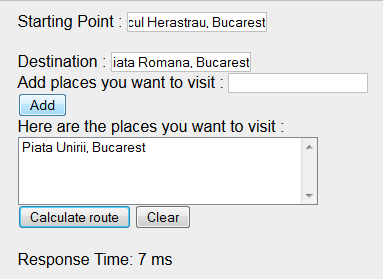
\includegraphics[scale=0.7]{input/make_route.png}
			\caption{\label{fig:route}How to use the application.}
		\end{figure}
		
		The route you should follow is displayed on the map after you clicked the \textit{Calculate} button. Markers are also used to show the points you want to pass by.
		
		\begin{figure}[h!]
			\centering
			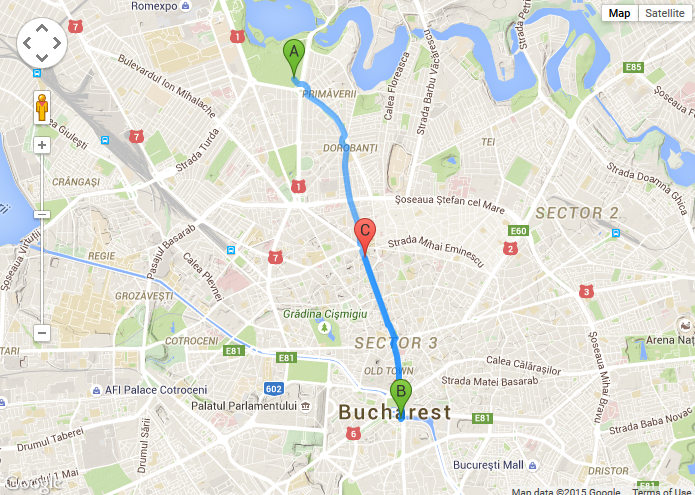
\includegraphics[scale=0.7]{input/map_result.png}
			\caption{\label{fig:map_result}Map displaying your optimized way through the points wanted.}
		\end{figure}
		
		As you can see, the directions are not visible by default, since they can be very long and detailed. The \textit{Display route instructions} link at the top of the map allows to display the route instructions for the tour. Since the application has been designed to visit a city, the directions will be for walking people, but you could eventually follow them with a bike. As you can see in \textsc{Figure} \ref{fig:instructions}, the directions have the basic features of Google Maps, like :
		
		\begin{enumerate}
			\item The approximate time travel to the next step;
			\item The distance between those steps;
			\item The distance to make between each instruction.
		\end{enumerate}
		
		\begin{figure}[h!]
			\centering
			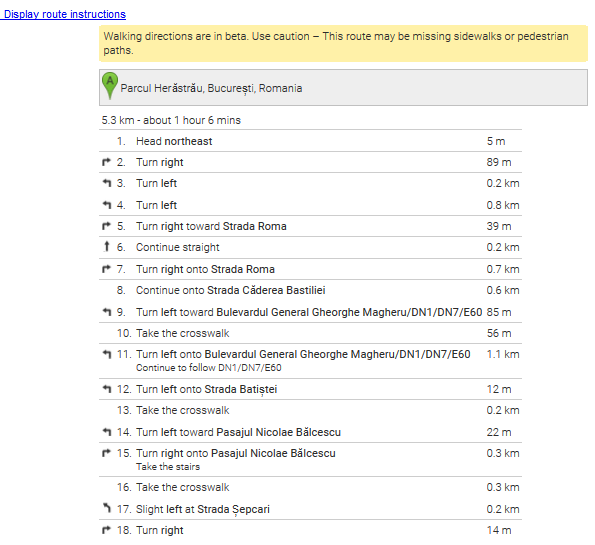
\includegraphics[scale=0.9]{input/instructions.png}
			\caption{\label{fig:instructions}You can display the specific directions.}
		\end{figure}
		
		\subsection{Technologies}

				\paragraph{Google Maps API and JavaScript}
				We mostly used the tools provided by the Google Maps API in our application. The Google Maps API is composed of a wide array of specialized APIs, dedicated to web pages, web services, and mobile applications. While, on the second step of our project, we mainly focused on the mobile API, we decided to implement a web page rather than a complete mobile application. The API dedicated to this task in the Google Maps API is the JavaScript API v3, so most of the code we wrote was JavaScript. Also, the statement we made in our previous report regarding the UI controls and customization of the maps are entirely valid in our implementation.
				To illustrate a basic utilization of the API, we will detail the main steps to create a map in a web page:
				\begin{itemize}
				\item{Load the API}: the API is loaded in the line :
					\textit{src="http://maps.googleapis.com/maps/api/js"};
				\item{Set the properties of the map}: the map is initialized at the beginning by this function:
				\begin{figure}[h!]
				\centering
				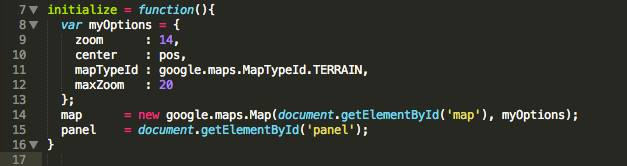
\includegraphics[scale=0.5]{input/map_code.jpg}
				\caption{Setting the map.}
				\label{fig:map_code}
				\end{figure}
				\end{itemize}
				The Map object that represents our map in the API is created by the constructor \newline \textit{google.maps.Map(document.getElementById("map"), map)} that takes as parameters the container of the map in the HTML file, and the set of properties we set in the \textit{initialize()} function.
				In our application, we also used the HTML5 geolocation integration in the API, and the calculation of directions. This calculation of the route and its drawing on the map is handled by this code:
				\begin{figure}[h!]
					\centering
					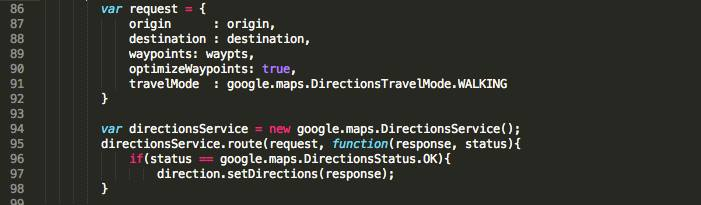
\includegraphics[scale=0.45]{input/directions_code.jpg}
					\caption{Request to calculate the route, and draw it on the map.}
					\label{fig:directions_code}
				\end{figure}
				\\
				In conclusion, all the tools regarding map generation, route calculation, time request calculation and directions computing are provided out-of-the-box by the Google Maps API in the form of JavaScript objects and functions.